\documentclass[tikz,border=2pt]{standalone}
\usepackage{amsmath,amssymb}
\usepackage{tikz}
\usetikzlibrary{arrows.meta}

\begin{document}
% Taxicab distance: travel along the grid, so d_1 = |Δx| + |Δy| (every staircase route has the
% same length), while the Euclidean distance is the straight diagonal.
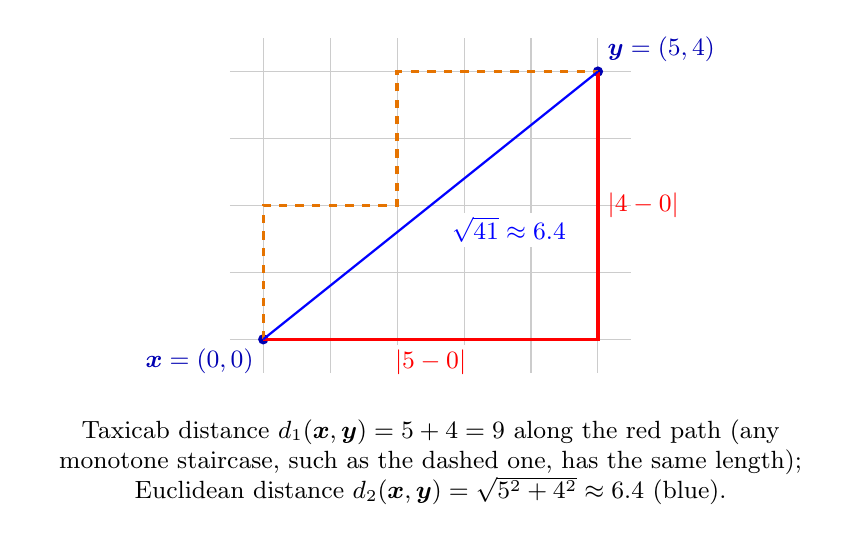
\begin{tikzpicture}[scale=0.85, every node/.style={font=\small}]
	\draw[gray!40, step=1] (-0.5,-0.5) grid (5.5,4.5);
	\fill[blue!70!black] (0,0) circle (2.2pt) node[below left] {$\boldsymbol{x}=(0,0)$};
	\fill[blue!70!black] (5,4) circle (2.2pt) node[above right] {$\boldsymbol{y}=(5,4)$};
	\draw[red, very thick] (0,0) -- (5,0) -- (5,4);
	\draw[orange!90!black, very thick, dashed] (0,0) -- (0,2) -- (2,2) -- (2,4) -- (5,4);
	\draw[blue, thick] (0,0) -- (5,4);
	\node[red, below, fill=white, inner sep=1.5pt, yshift=-2pt] at (2.5,0) {$|5-0|$};
	\node[red, right] at (5,2) {$|4-0|$};
	\node[blue, anchor=north west, fill=white, inner sep=1.5pt] at (2.75,1.9) {$\sqrt{41}\approx 6.4$};
	\node[anchor=north, align=flush center, text width=10cm] at (2.5,-1.05) {Taxicab distance $d_1(\boldsymbol{x},\boldsymbol{y})=5+4=9$ along the red path (any monotone staircase, such as the dashed one, has the same length); Euclidean distance $d_2(\boldsymbol{x},\boldsymbol{y})=\sqrt{5^2+4^2}\approx 6.4$ (blue).};
\end{tikzpicture}
\end{document}
